
\subsection{Datasets and Training and Testing}
We collect over $8$M data from 11 public datasets for training. Datasets are listed in Tab.~\ref{table: datasets}. The autonomous driving datasets, including DDAD~\cite{packnet}, Lyft~\cite{lyftl5preception}, DrivingStereo~\cite{yang2019drivingstereo}, Argoverse2~\cite{Argoverse2}, DSEC~\cite{Gehrig21ral}, and Pandaset~\cite{itsc21pandaset}, have provided LiDar and camera intrinsic and extrinsic parameters. We project the LiDar to image planes to obtain ground-truth depths. In contrast, Cityscapes~\cite{Cordts2016Cityscapes}, DIML~\cite{cho2021diml}, and UASOL~\cite{bauer2019uasol} only provide calibrated stereo images. We use draftstereo~\cite{lipson2021raft} to achieve pseudo ground-truth depths. Mapillary PSD~\cite{MapillaryPSD} dataset provides paired RGB-D, but the depth maps are achieved from a structure-from-motion method. The camera intrinsic parameters are estimated from the SfM. We believe that such achieved metric information is noisy. Thus we do not enforce learning-metric-depth loss on this data, \textit{i.e.},  $L_{silog}$, to reduce the effect of noises. For the Taskonomy~\cite{zamir2018taskonomy} dataset, we follow LeReS~\cite{yin2022towards} to obtain the instance planes, which are employed in the pair-wise normal regression loss. During training, we employ the training strategy from \cite{yin2020diversedepth_old} to balance all datasets in each training batch. 

The testing data is listed in Tab.~\ref{table: datasets}. All of them are captured by high-quality sensors. In testing, we employ their provided camera intrinsic parameters to perform our proposed canonical space transformation. 



\begin{table}[]
\caption{Training and testing datasets used in experiments.}
\vspace{-1 em}
\centering
\begin{threeparttable}
\scalebox{0.8}{
\begin{tabular}{ r llll}
 \toprule[1pt]
\multicolumn{1}{l|}{Datasets}                       & \multicolumn{1}{l|}{Scenes}         & \multicolumn{1}{l|}{%
Label}              & \multicolumn{1}{l|}{Size}        & \# Cam.  \\ \hline
\multicolumn{5}{c}{Training Data}                                                                                                                                                          \\ \hline
\multicolumn{1}{l|}{DDAD~\cite{packnet}}                           & \multicolumn{1}{l|}{Outdoor}        & \multicolumn{1}{l|}{LiDar}                 & \multicolumn{1}{l|}{$\sim$80K}   & 36+            \\
\multicolumn{1}{l|}{Lyft~\cite{lyftl5preception}}                           & \multicolumn{1}{l|}{Outdoor}        & \multicolumn{1}{l|}{LiDar}                 & \multicolumn{1}{l|}{$\sim$50K}   & 6+             \\
\multicolumn{1}{l|}{Driving Stereo (DS)~\cite{yang2019drivingstereo}}                 & \multicolumn{1}{l|}{Outdoor}        & \multicolumn{1}{l|}{Stereo\tnote{\dag}}       & \multicolumn{1}{l|}{$\sim$181K}  & 1              \\
\multicolumn{1}{l|}{DIML~\cite{cho2021diml}}                           & \multicolumn{1}{l|}{Outdoor}        & \multicolumn{1}{l|}{Stereo\tnote{\dag}}       & \multicolumn{1}{l|}{$\sim$122K}  & 10             \\
\multicolumn{1}{l|}{Arogoverse2~\cite{Argoverse2}}                    & \multicolumn{1}{l|}{Outdoor}        & \multicolumn{1}{l|}{LiDar}                 & \multicolumn{1}{l|}{$\sim$3515K} & 6+             \\
\multicolumn{1}{l|}{Cityscapes~\cite{Cordts2016Cityscapes}}                     & \multicolumn{1}{l|}{Outdoor}        & \multicolumn{1}{l|}{Stereo\tnote{\dag}}       & \multicolumn{1}{l|}{$\sim$170K}  & 1              \\
\multicolumn{1}{l|}{DSEC~\cite{Gehrig21ral}}                           & \multicolumn{1}{l|}{Outdoor}        & \multicolumn{1}{l|}{LiDar}                 & \multicolumn{1}{l|}{$\sim$26K}   & 1              \\
\multicolumn{1}{l|}{Mapillary PSD~\cite{MapillaryPSD}} & \multicolumn{1}{l|}{Outdoor}        & \multicolumn{1}{l|}{SfM\tnote{\ddag}} & \multicolumn{1}{l|}{750K}        & 1000+          \\
\multicolumn{1}{l|}{Pandaset~\cite{itsc21pandaset}}                       & \multicolumn{1}{l|}{Outdoor}        & \multicolumn{1}{l|}{LiDar}                 & \multicolumn{1}{l|}{$\sim$48K}         & 6              \\
\multicolumn{1}{l|}{UASOL~\cite{bauer2019uasol}}                          & \multicolumn{1}{l|}{Outdoor}        & \multicolumn{1}{l|}{Stereo\tnote{\dag}}       & \multicolumn{1}{l|}{$\sim$137K}        & 1              \\
\multicolumn{1}{l|}{Taskonomy~\cite{zamir2018taskonomy}}                      & \multicolumn{1}{l|}{Indoor}         & \multicolumn{1}{l|}{LiDar}                 & \multicolumn{1}{l|}{$\sim$4M}       & $\sim$1M            \\ \hline
\multicolumn{5}{c}{Testing Data}                                                                                                                                                           \\ \hline
\multicolumn{1}{l|}{NYU~\cite{silberman2012indoor}}                            & \multicolumn{1}{l|}{Indoor}         & \multicolumn{1}{l|}{Kinect}                & \multicolumn{1}{l|}{654}         & 1              \\
\multicolumn{1}{l|}{KITTI~\cite{Geiger2013IJRR}}                          & \multicolumn{1}{l|}{Outdoor}        & \multicolumn{1}{l|}{LiDar}                 & \multicolumn{1}{l|}{652}           & 4         \\
\multicolumn{1}{l|}{ScanNet~\cite{dai2017scannet}}                        & \multicolumn{1}{l|}{Indoor}         & \multicolumn{1}{l|}{Kinect}                & \multicolumn{1}{l|}{700}         & 1              \\
\multicolumn{1}{l|}{NuScenes (NS)~\cite{caesar2020nuscenes}}                       & \multicolumn{1}{l|}{Outdoor}        & \multicolumn{1}{l|}{LiDar}                 & \multicolumn{1}{l|}{10K}           & 6              \\
\multicolumn{1}{l|}{ETH3D~\cite{schops2017multi}}                          & \multicolumn{1}{l|}{Outdoor}        & \multicolumn{1}{l|}{LiDar}                 & \multicolumn{1}{l|}{431}           & 1              \\
\multicolumn{1}{l|}{DIODE~\cite{vasiljevic2019diode}}                          & \multicolumn{1}{l|}{In/Out} & \multicolumn{1}{l|}{LiDar}                 & \multicolumn{1}{l|}{771}           & 1           \\
\multicolumn{1}{l|}{7Scenes~\cite{shotton2013scene}}                        & \multicolumn{1}{l|}{Indoor}         & \multicolumn{1}{l|}{Kinect}                & \multicolumn{1}{l|}{17k}           & 1              \\
\multicolumn{1}{l|}{iBims-1~\cite{koch2018evaluation}}                        & \multicolumn{1}{l|}{Indoor}         & \multicolumn{1}{l|}{LiDar}                & \multicolumn{1}{l|}{100}           & 1              \\
\toprule[1pt]
\end{tabular}}
\begin{tablenotes}
\footnotesize
\item[\dag]`Stereo': we use RaftStereo~\cite{lipson2021raft} to retrieve the pseudo ground truth.
\item[\ddag]`SfM': pseudo ground truth is retrieved by structure from motion.
\end{tablenotes}
\end{threeparttable}
\label{table: datasets}
\end{table}

\subsection{Details for Some Experiments}
\noindent\textbf{Evaluation of zero-shot 3D scene reconstruction.} In this experiment, we use all methods' released models to predict each frame's depth and use the ground-truth poses and camera intrinsic parameters to reconstruct point clouds. When evaluating the reconstructed point cloud, we employ the iterative closest point (ICP)~\cite{besl1992method} algorithm to match the predicted point clouds with ground truth by a pose transformation matrix. Finally, we evaluate the Chamfer $\ell_1$ distance and F-score on the point cloud.

\noindent\textbf{Reconstruction of in-the-wild scenes.} We collect several photos from Flickr. From their associated camera metadata, we can obtain the focal length $\hat{f}$ and the pixel size $\delta$. According to $\nicefrac{\hat{f}}{\delta}$, we can obtain the pixel-represented focal length for 3D reconstruction and achieve the metric information. We use meshlab software to measure some structures' size on point clouds. More visual results are shown in Fig. \ref{fig: recon in the wild.}.

\noindent\textbf{Generalization of metric depth estimation.} To evaluate our method's robustness of metric recovery, we test on 8 zero-shot datasets, i.e. NYU, KITTI, DIODE (indoor and outdoor parts), ETH3D, iBims-1, NuScenes, and 7Scenes. Details are reported in Tab.~\ref{table: datasets}.  We use the officially provided focal length to predict the metric depths. All benchmarks use the same depth model for evaluation. We don't perform any scale alignment.  

\noindent\textbf{Evaluation on affine-invariant depth benchmarks.} We follow existing affine-invariant depth estimation methods to evaluate 5 zero-shot datasets. Before evaluation, we employ the least square fitting to align the scale and shift with ground truth~\cite{leres}. Previous methods' performance is cited from their papers. 

\noindent\textbf{Dense-SLAM Mapping.} This experiment is conducted on the KITTI odometry benchmark. We use our model to predict metric depths, and then naively input them to the Droid-SLAM system as an initial depth. We do not perform any finetuning but directly run their released codes on KITTI. With Droid-SLAM predicted poses, we unproject depths to the 3D point clouds and fuse them together to achieve dense metric mapping. More qualitative results are shown in Fig.~\ref{fig: dense_slam1.}.


\subsection{More Visual Results}
\noindent\textbf{Reconstructing 360\degree NuScenes scenes.} Current autonomous driving cars are equipped with several pin-hole cameras to capture 360\degree views. Capturing the surround-view depth is important for autonomous driving.  We sampled some scenes from the testing data of NuScenes. With our depth model, we can obtain the metric depths for 6-ring cameras. With the provided camera intrinsic and extrinsic parameters, we unproject the depths to the 3D point cloud and merge all views together. See Fig. \ref{fig: recon nuscenes.} for details. Note that 6-ring cameras have different camera intrinsic parameters. We can observe that all views' point clouds can be fused together consistently.


\noindent\textbf{Qualitative comparison of depth estimation.} In Figs.~\ref{fig: depth_cmp1.},~\ref{fig: depth_cmp2.},~\ref{fig: depth_cmp3.}, and ~\ref{fig: depth_cmp4.}, We show the qualitative comparison of depth maps with Adabins~\cite{bhat2021adabins}, NewCRFs~\cite{yuan2022new}, and Omnidata~\cite{eftekhar2021omnidata}. Our results have much less artifacts.

\begin{figure*}[]
\centering
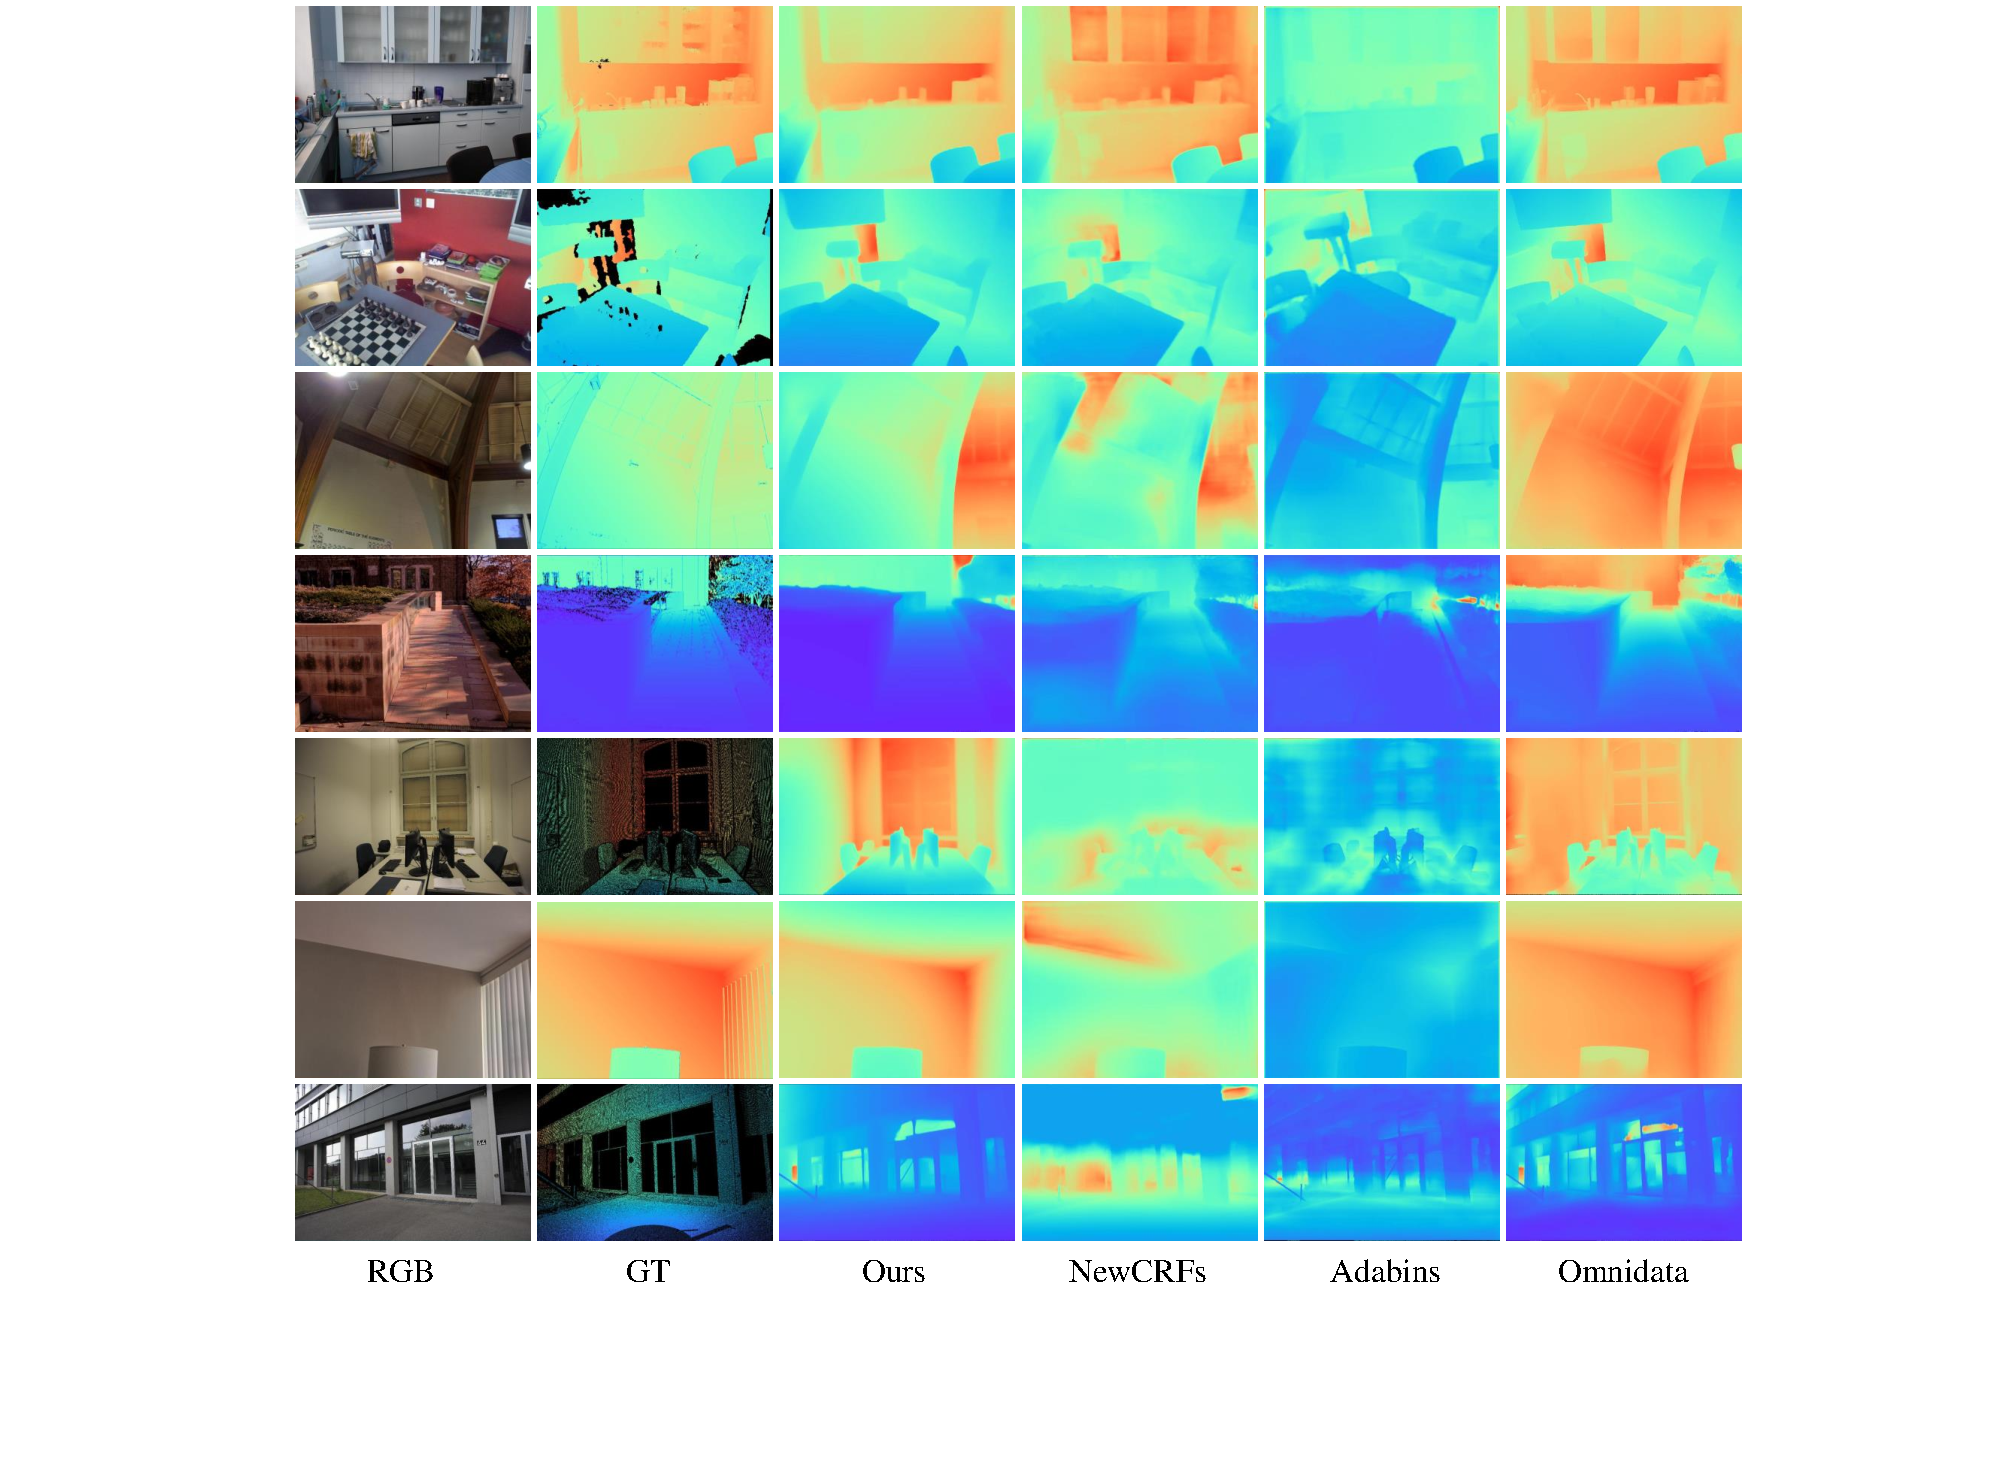
\includegraphics[width=1\textwidth]{./files/supp_depth_1.pdf}
\caption{\textbf{Depth estimation.} The visual comparison of predicted on iBims, ETH3D, and DIODE.}
\label{fig: depth_cmp1.}
\end{figure*}



\begin{figure*}[]
\centering
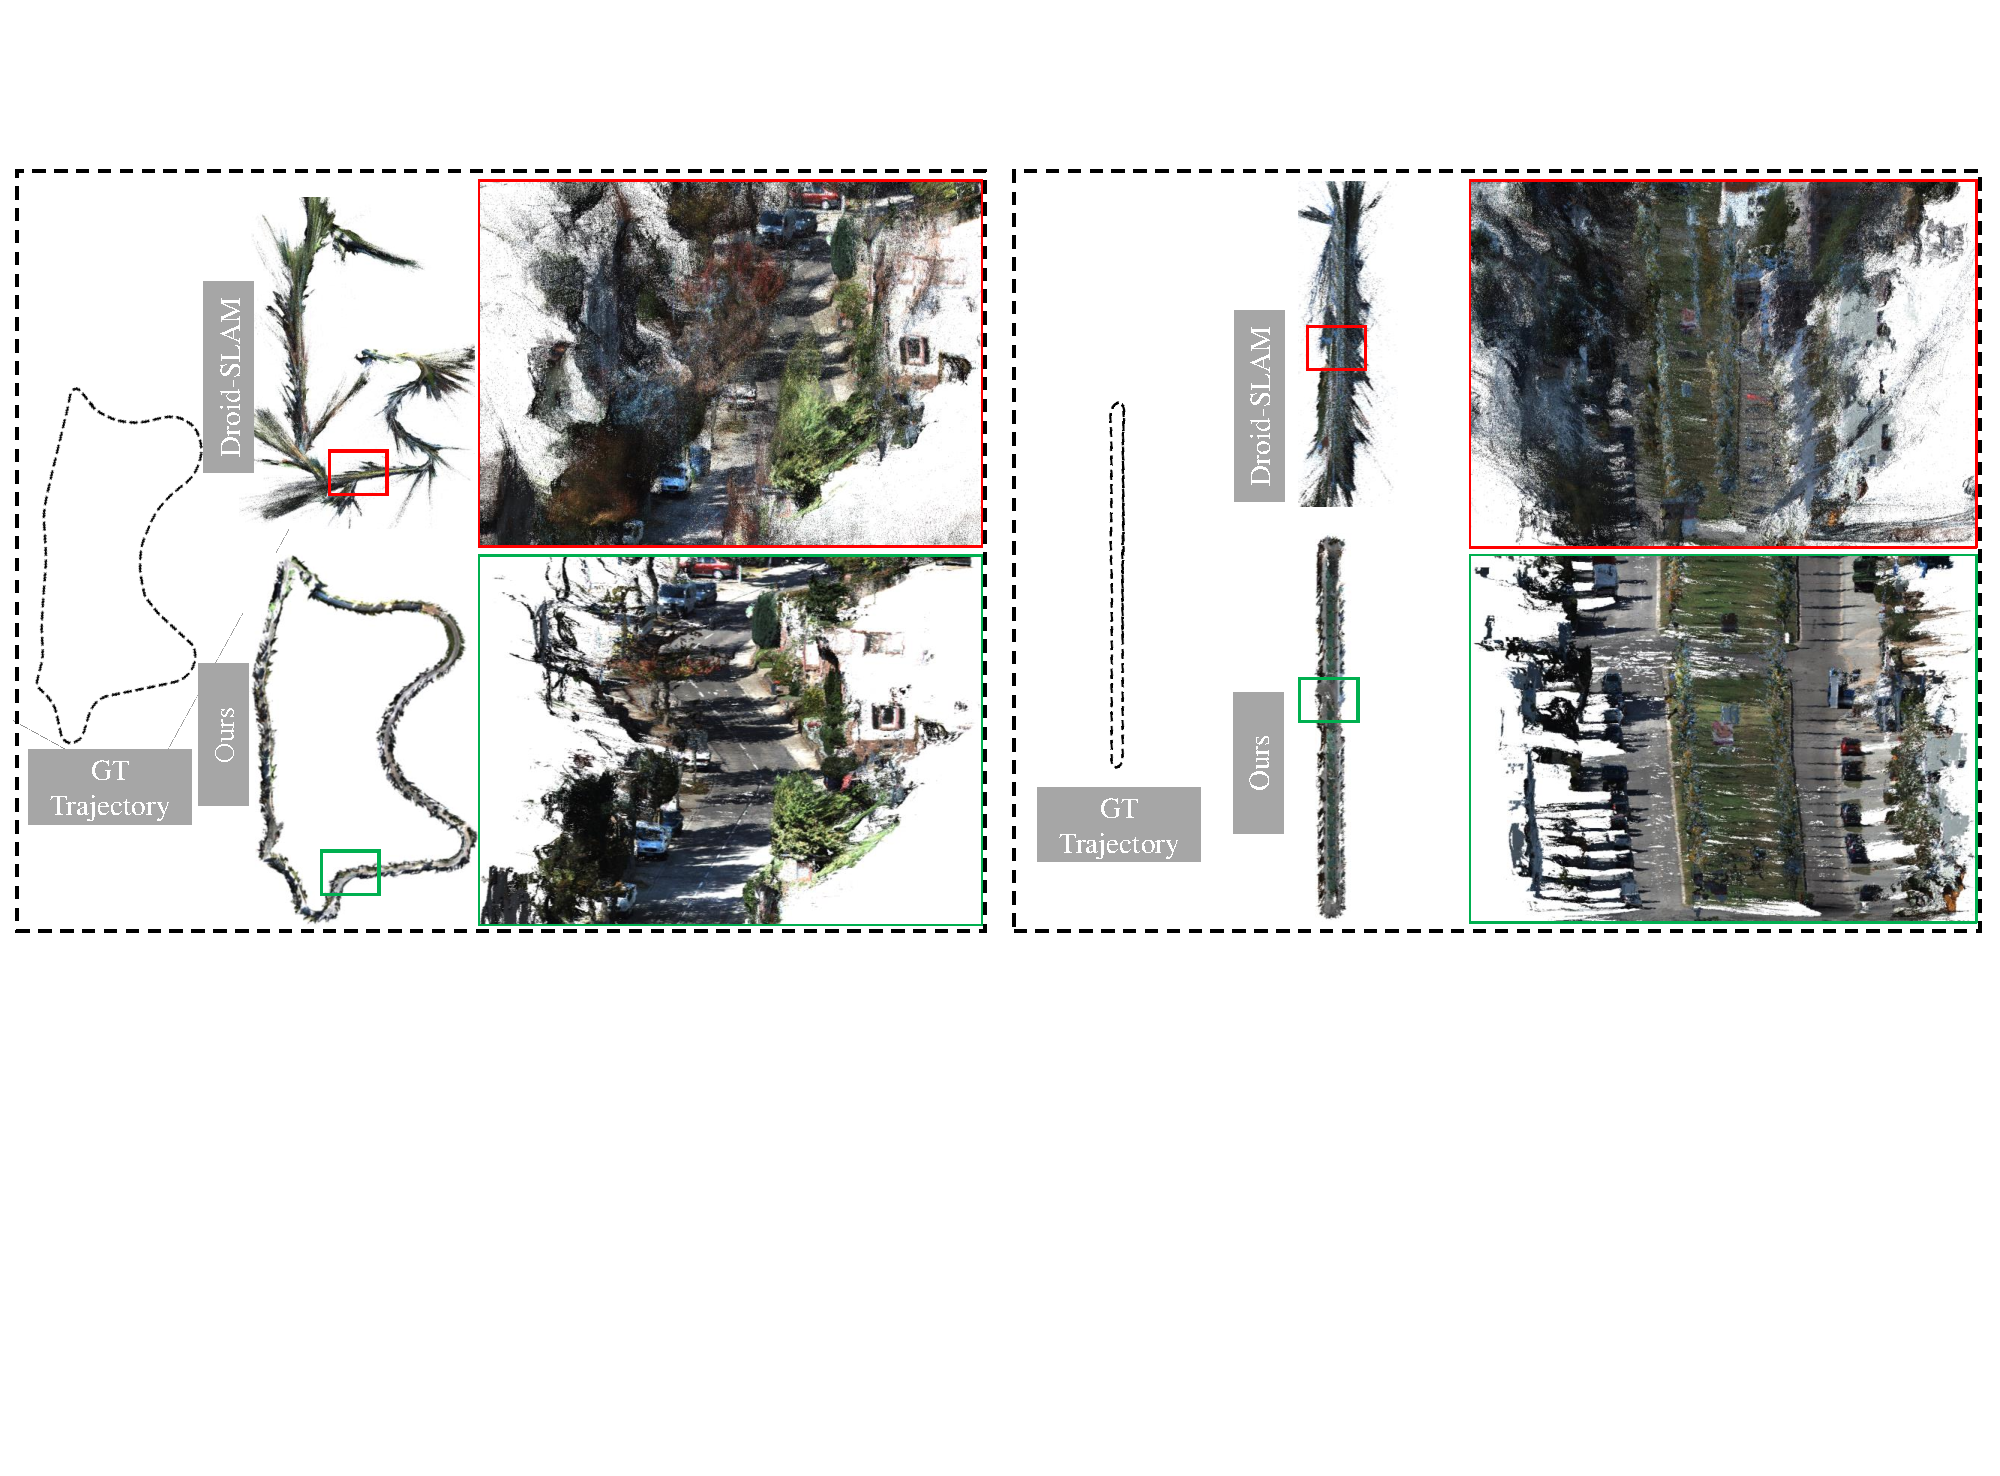
\includegraphics[width=0.95\textwidth]{./files/supp_slam1.pdf}
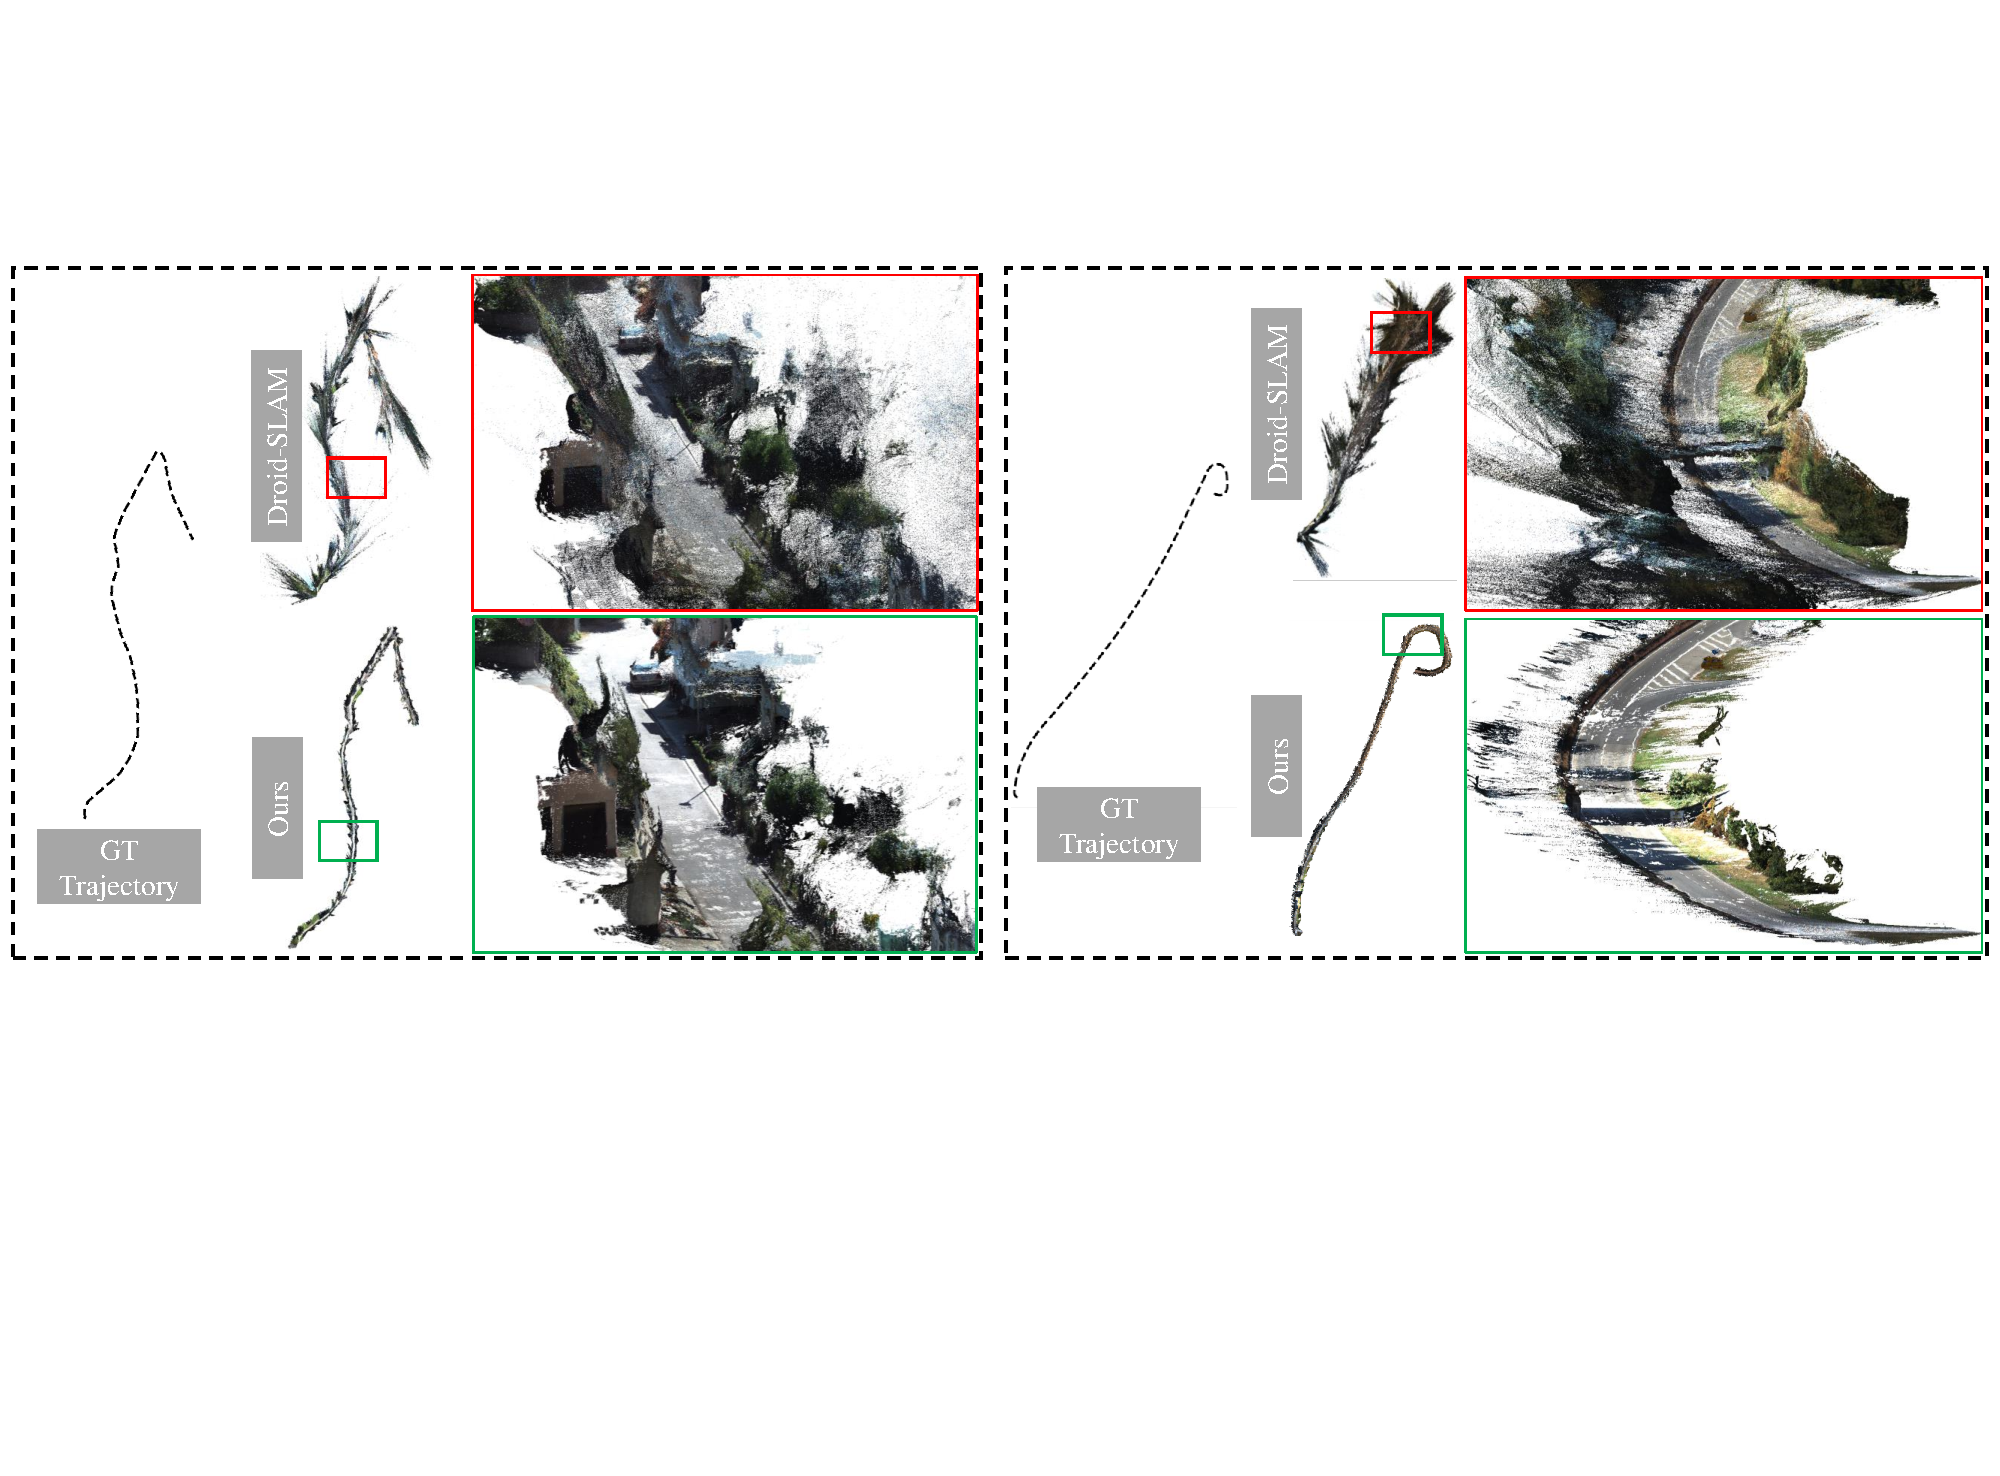
\includegraphics[width=0.95\textwidth]{./files/supp_slam2.pdf}
\caption{\textbf{Dense-SLAM Mapping.} Existing SOTA mono-SLAM methods usually face scale drift problems in large-scale scenes and are unable to achieve the metric scale. We show the ground-truth trajectory and Droid-SLAM~\cite{teed2021droid} predicted trajectory and their dense mapping. Then, we naively input our metric depth to Droid-SLAM, which can recover a much more accurate trajectory and perform the \textit{metric} dense mapping. }
\label{fig: dense_slam1.}
\end{figure*}


\begin{figure*}[]
\centering
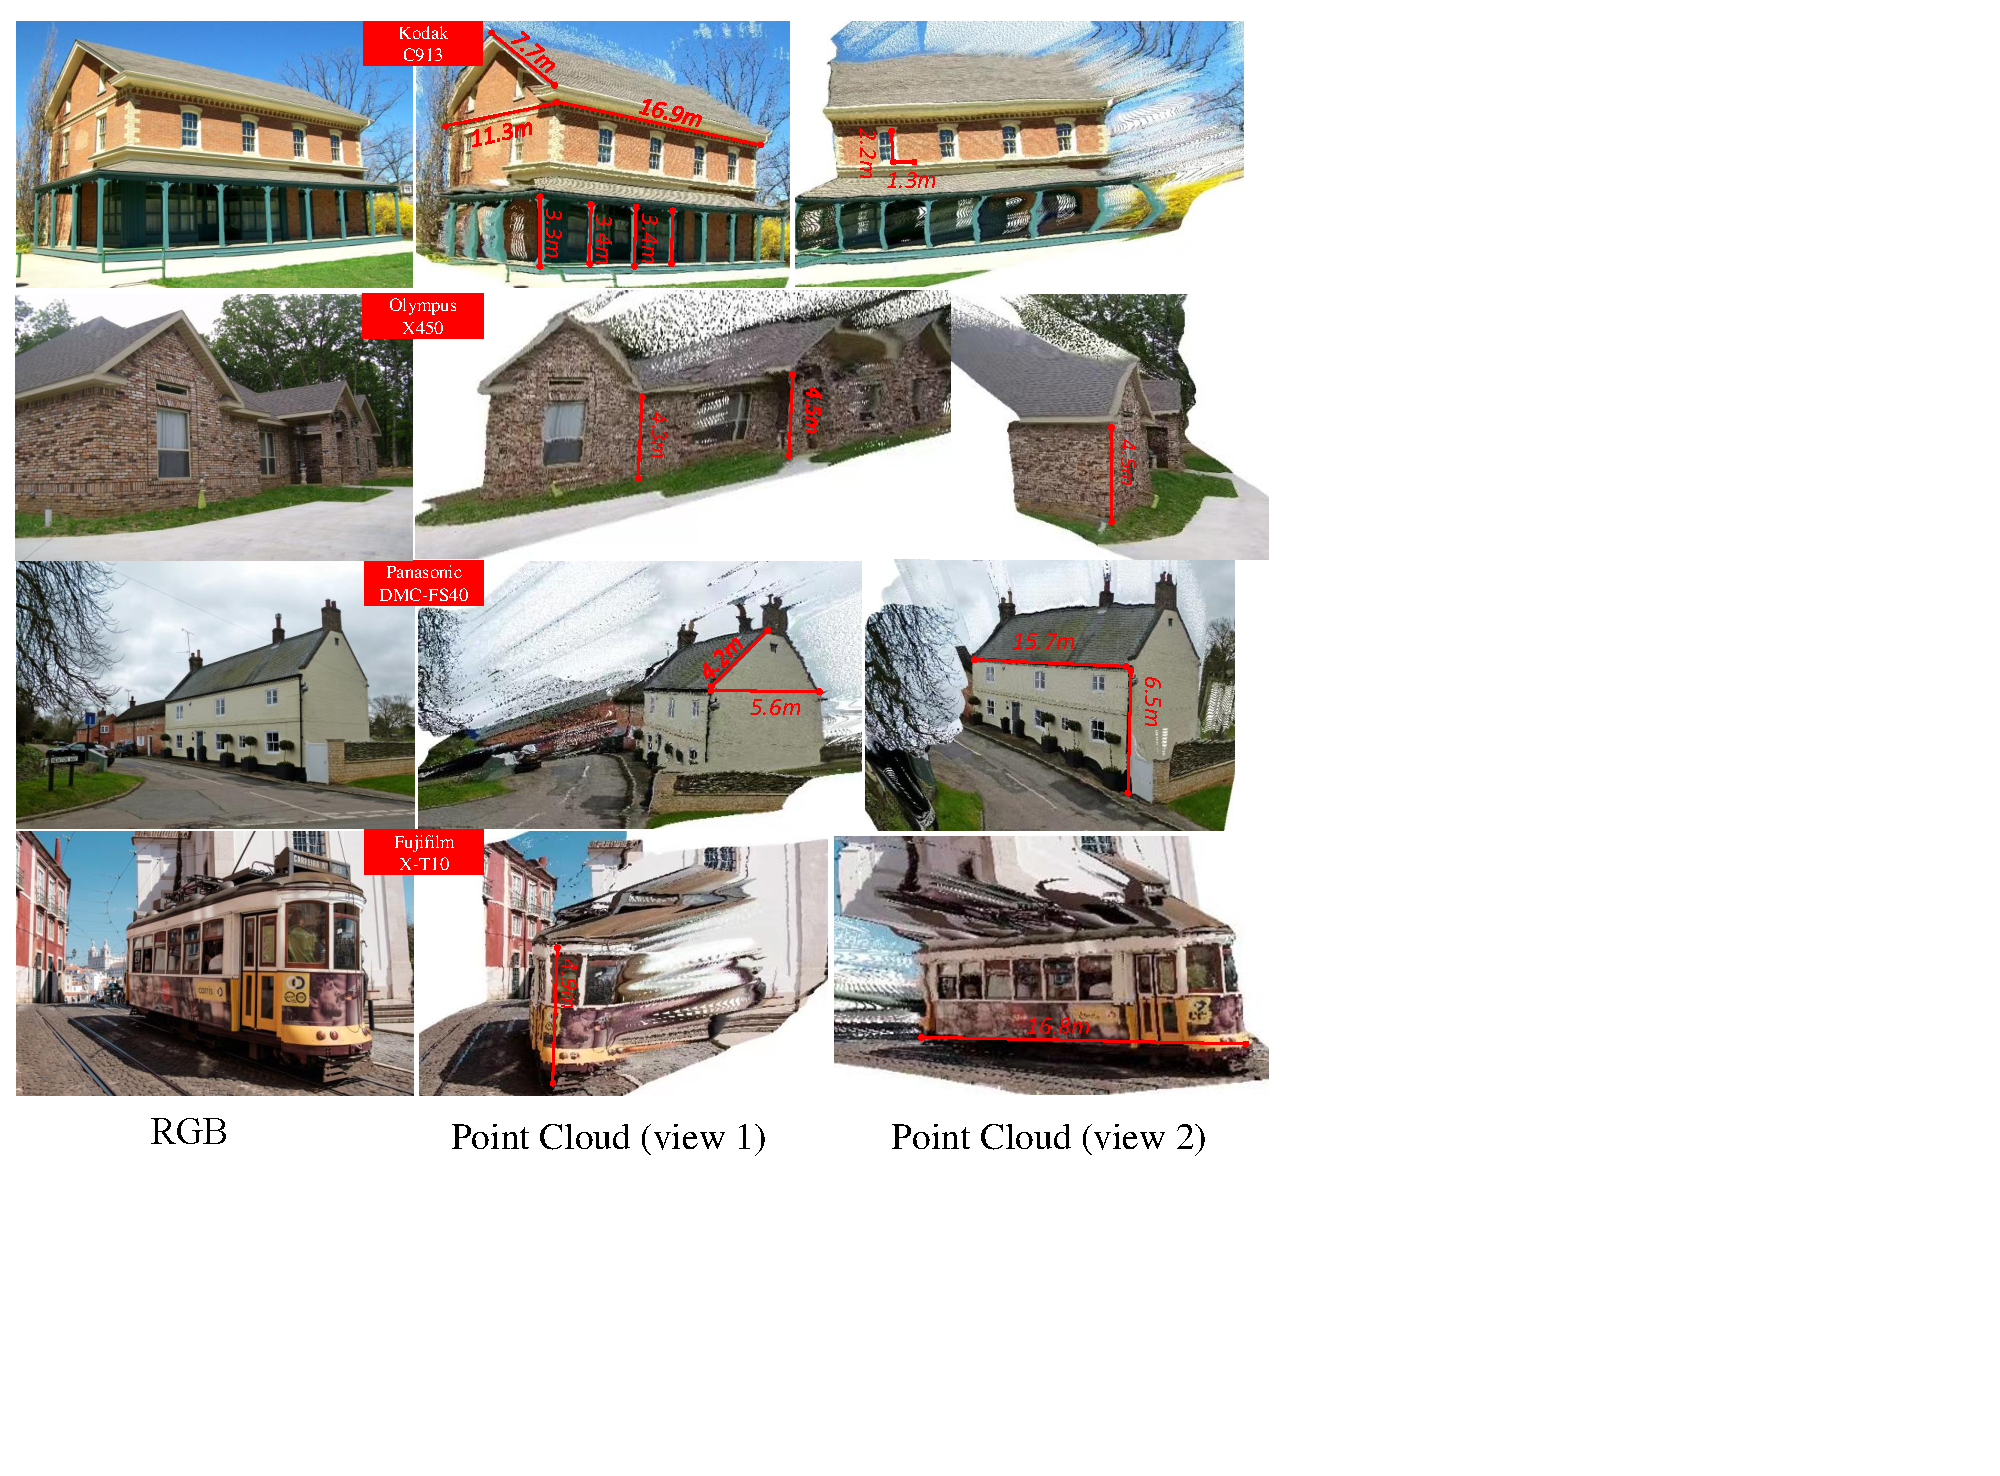
\includegraphics[width=0.8\textwidth]{./files/supp_in_the_wild.pdf}
\caption{\textbf{3D metric reconstruction of in-the-wild images.} We collect several Flickr images and use our model to reconstruct the scene. The focal length information is collected from the photo's metadata. From the reconstructed point cloud, we can measure some structures' sizes. We can observe that sizes are in a reasonable range. }
\label{fig: recon in the wild.}
\end{figure*}


\begin{figure*}[]
\centering
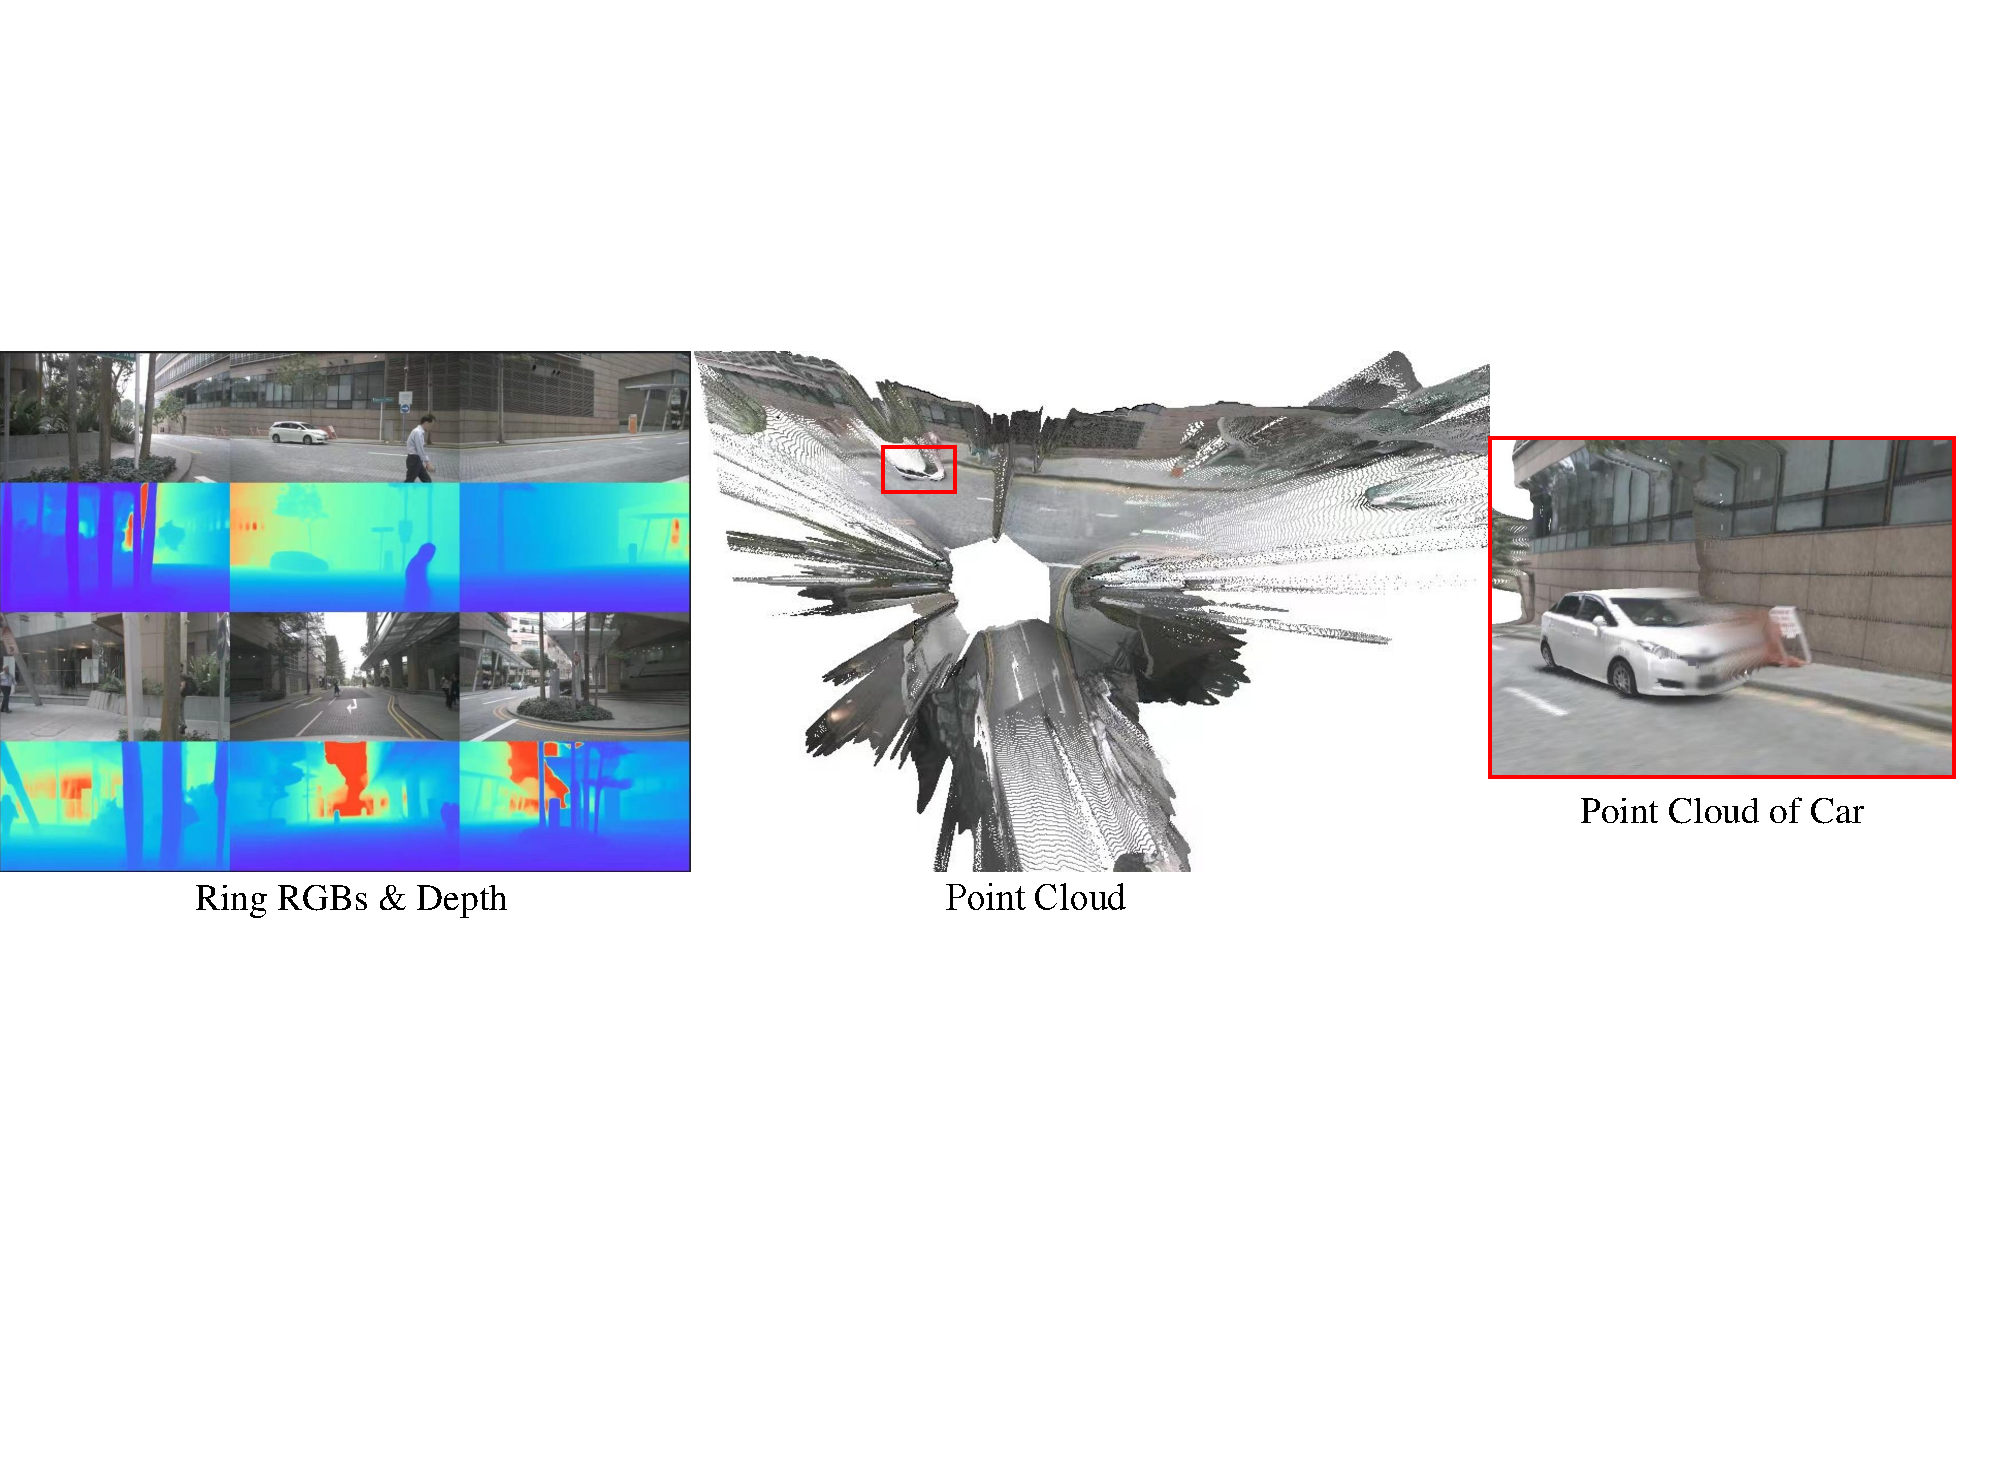
\includegraphics[width=1\textwidth]{./files/supp_nuscenes_ring2.pdf}
\caption{\textbf{3D reconstruction of 360\degree views.} Current autonomous driving cars are equipped with several pin-hole cameras to capture 360\degree views. With our model, we can reconstruct each view and smoothly fuse them together. We can see that all views can be well merged together without scale inconsistency problems. Testing data are from NuScenes. Note that the front view camera has a different focal length from other views. }
\label{fig: recon nuscenes.}
\end{figure*}


\begin{figure*}[]
\centering
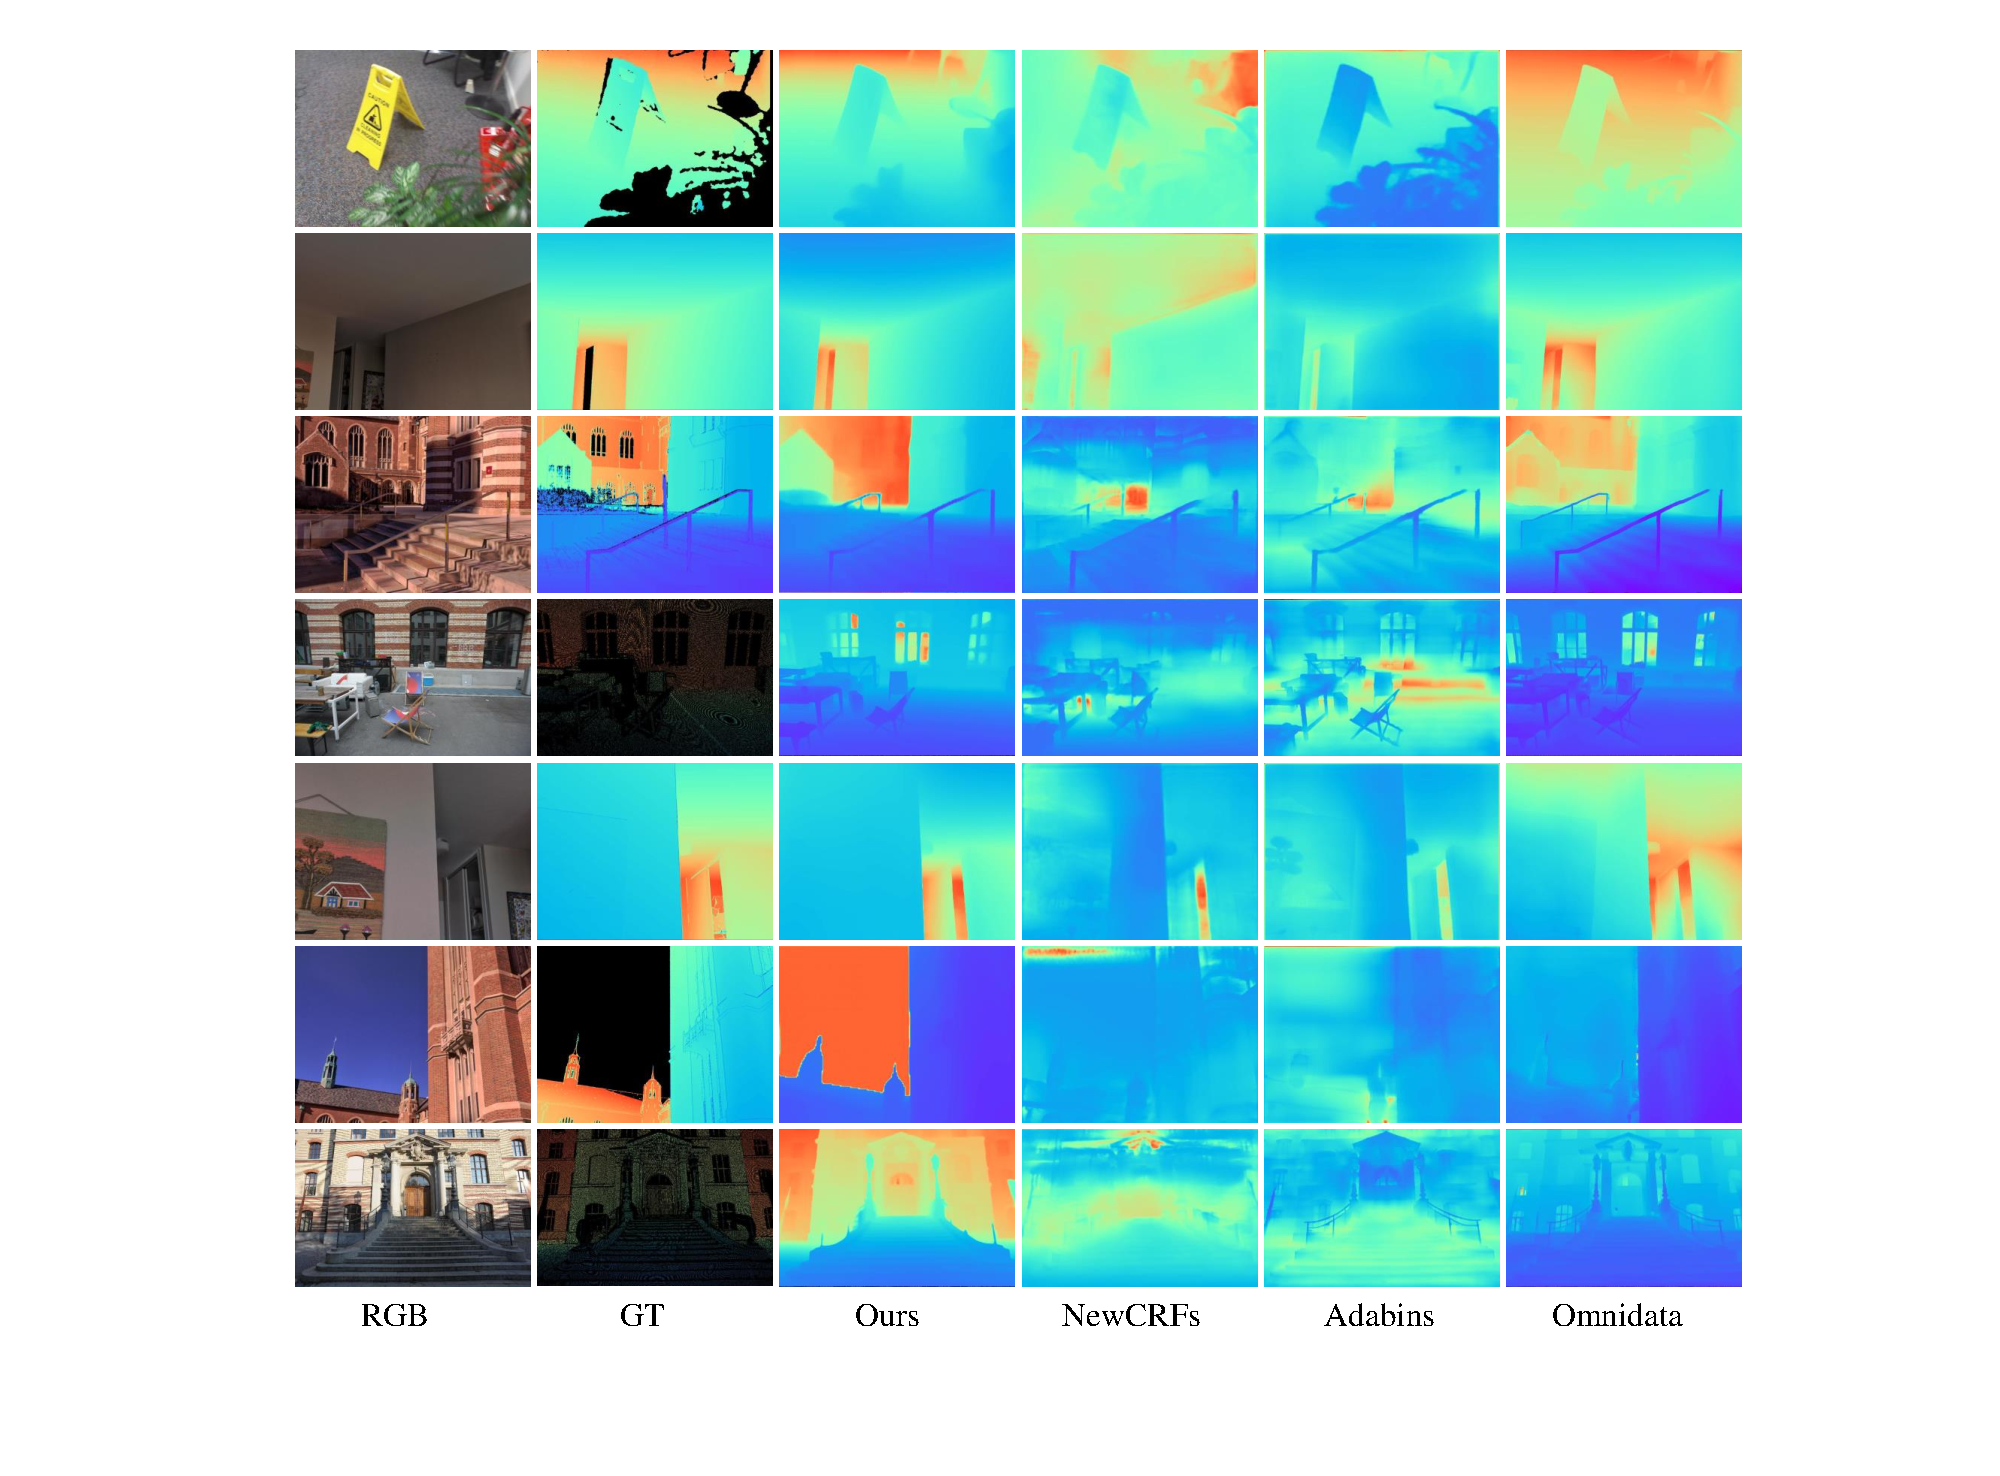
\includegraphics[width=0.9\textwidth]{./files/supp_depth_2.pdf}
\caption{\textbf{Depth estimation.} The visual comparison of predicted on iBims, ETH3D, and DIODE.}
\label{fig: depth_cmp2.}
\end{figure*}

\begin{figure*}[]
\centering
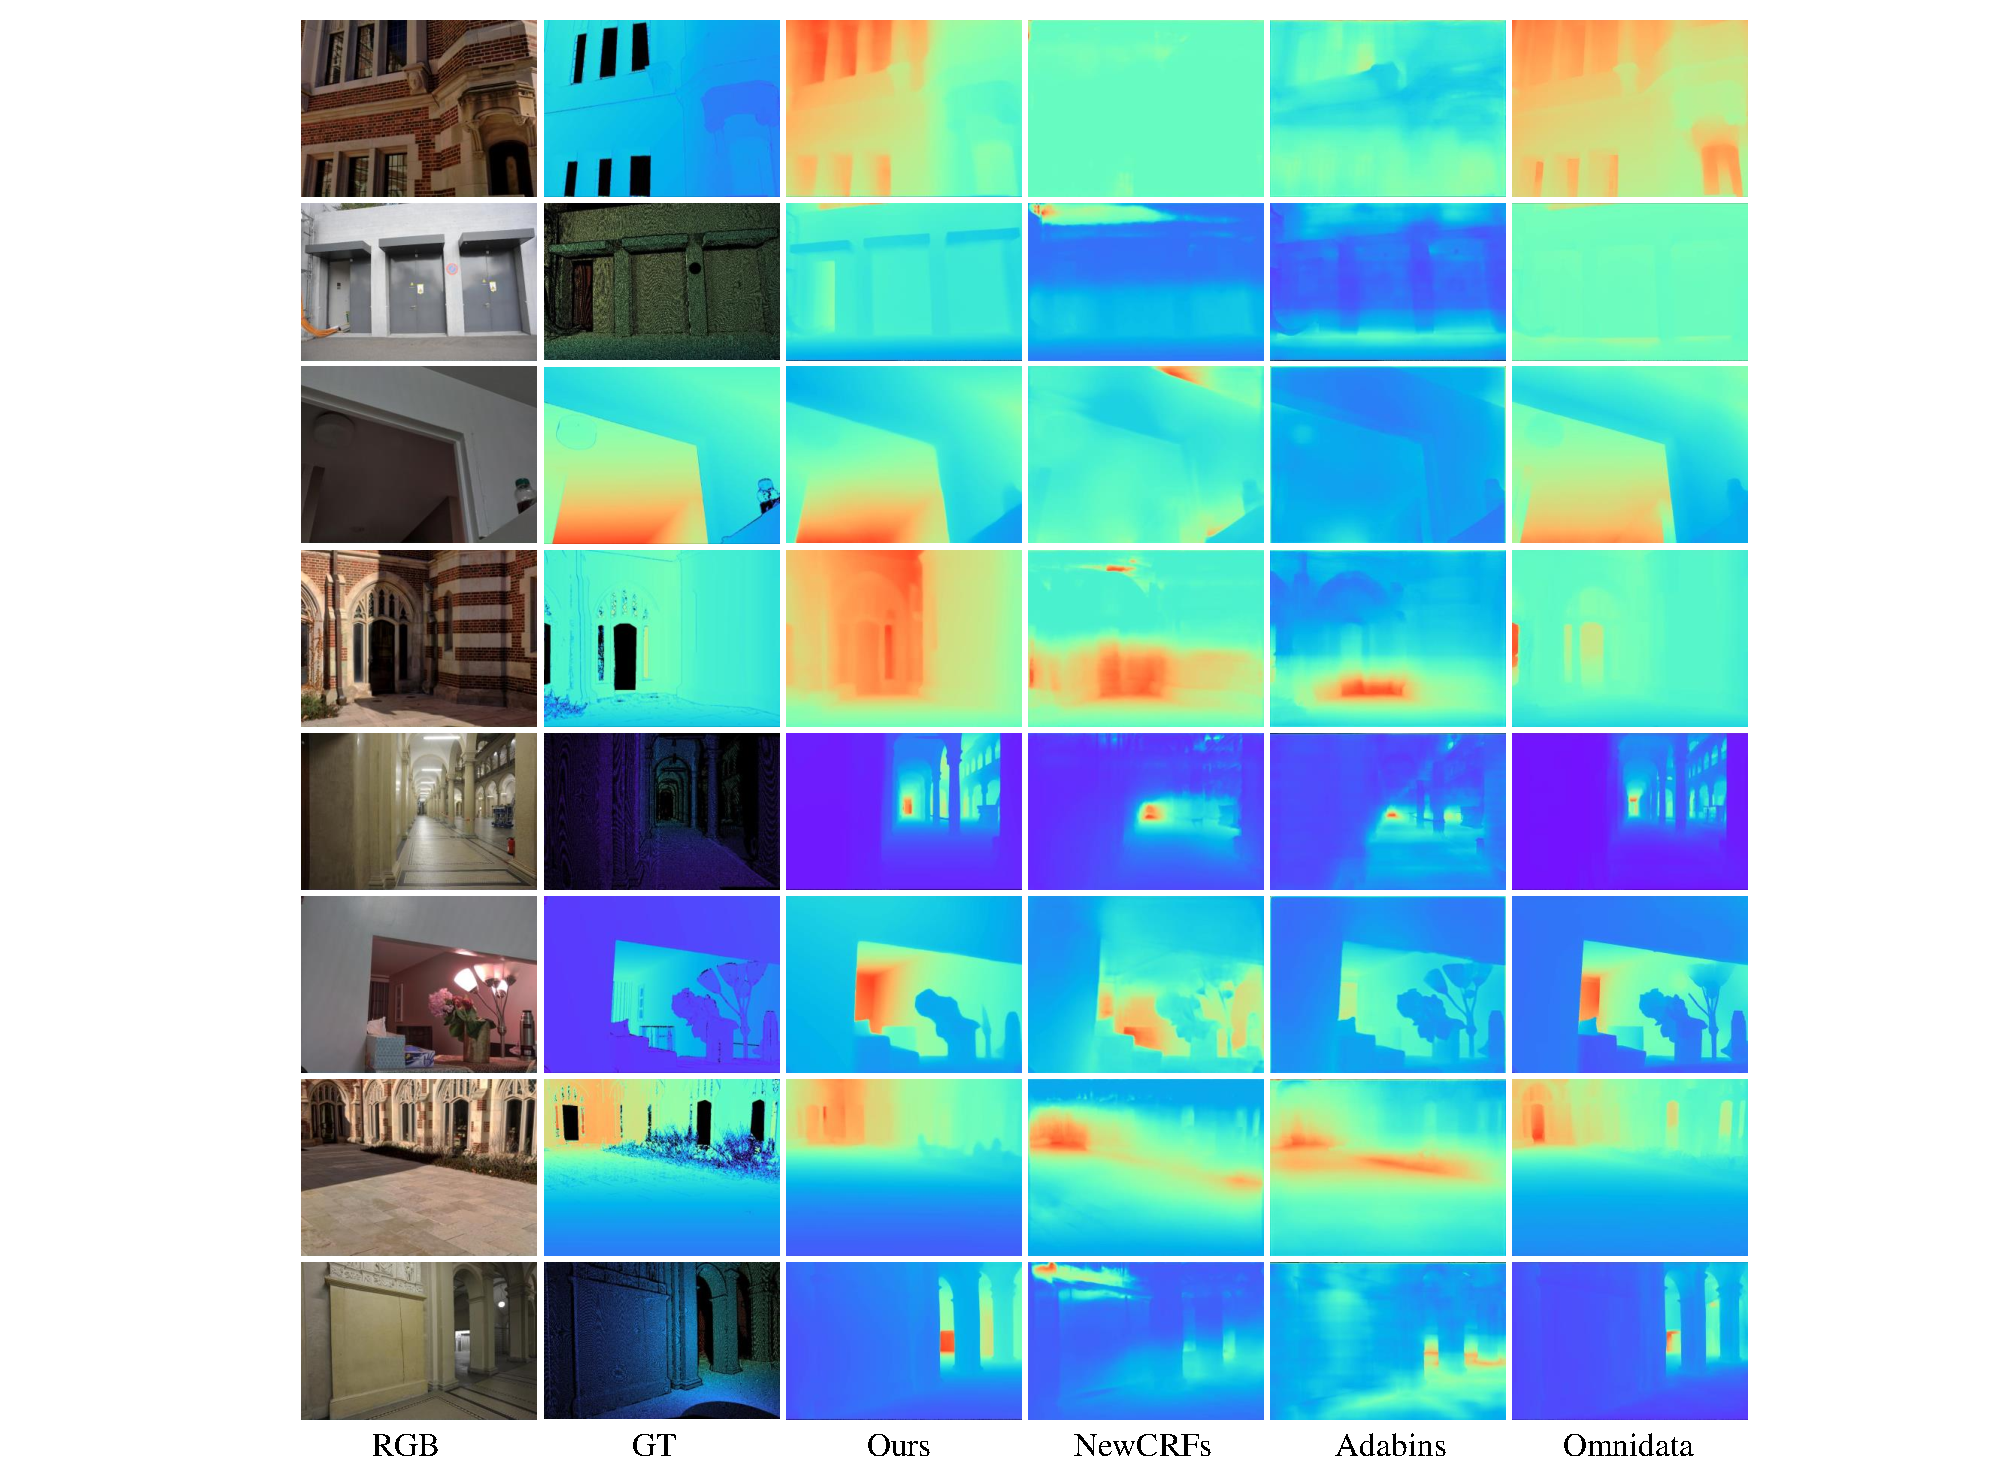
\includegraphics[width=0.9\textwidth]{./files/supp_depth_3.pdf}
\caption{\textbf{Depth estimation.} The visual comparison of predicted on iBims, ETH3D, and DIODE.}
\label{fig: depth_cmp3.}
\end{figure*}

\begin{figure*}[]
\centering
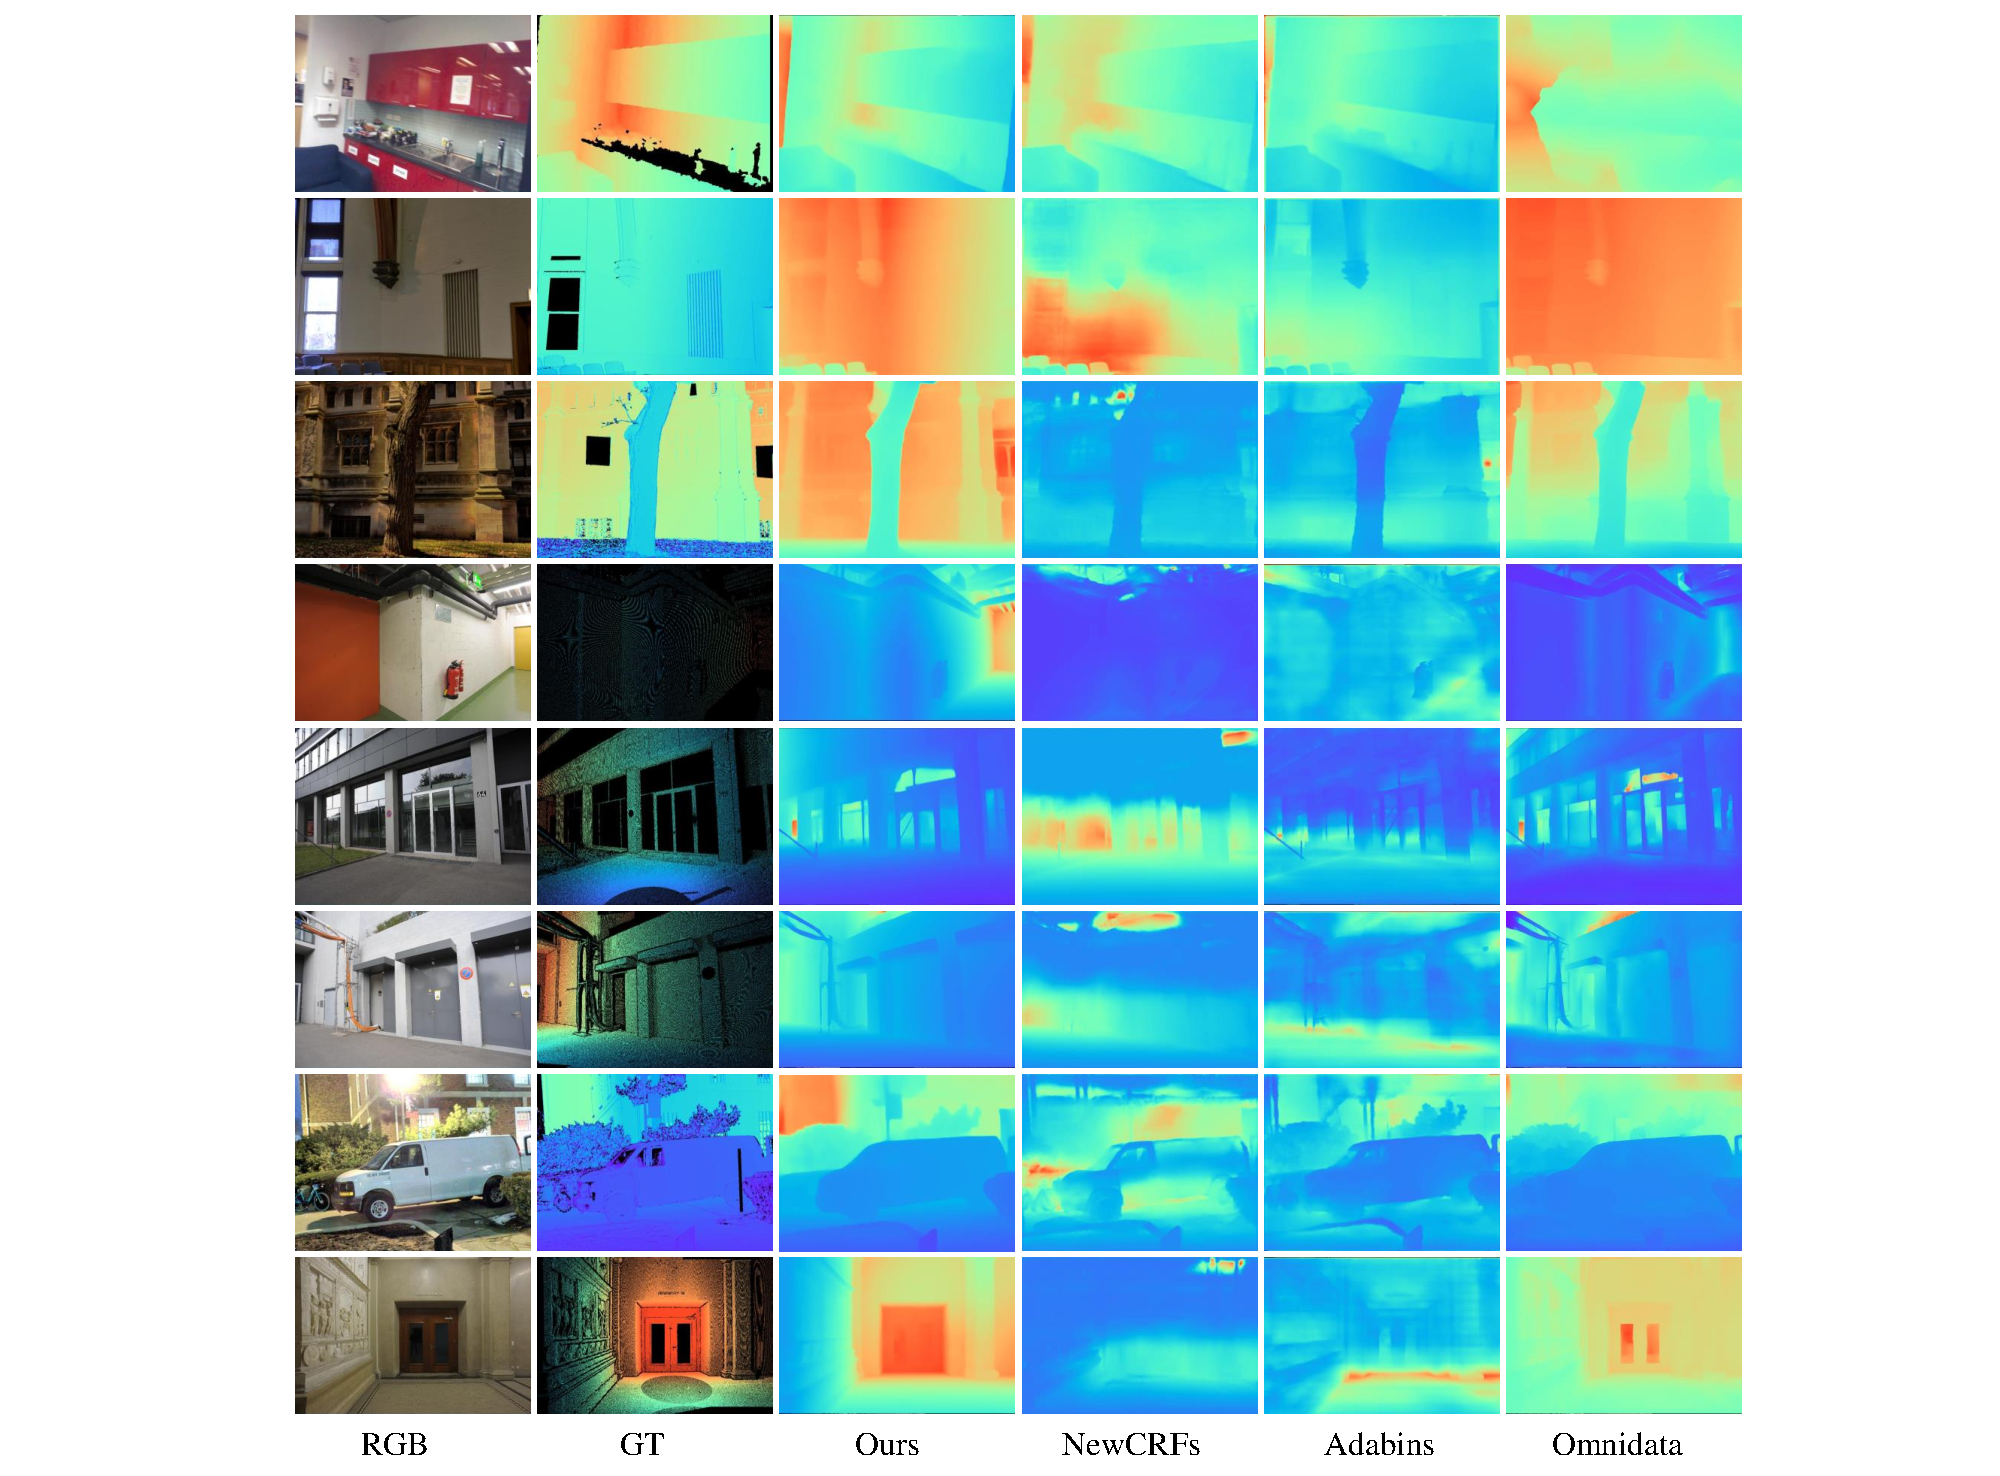
\includegraphics[width=0.9\textwidth]{./files/supp_depth_4.pdf}
\caption{\textbf{Depth estimation.} The visual comparison of predicted on iBims, ETH3D, and DIODE.}
\label{fig: depth_cmp4.}
\end{figure*}
